\problemname{The Photographer}
A photographer has taken many nice photos with their digital camera and connects it
to their computer to transfer the images. The images were taken with different rotations
of the camera so now some of the images are rotated. We call the four possible
rotations a photo can have \emph{up}, \emph{right}, \emph{down}, and \emph{left} and
define it as the side that corresponds to upward in the image. An image is correctly oriented
if it is rotated \emph{up}. The computer displays the images in a list and has a function
that rotates an image $90^\circ$ clockwise. The rotation thus follows this order:

\begin{figure}[h!]
    \centering
    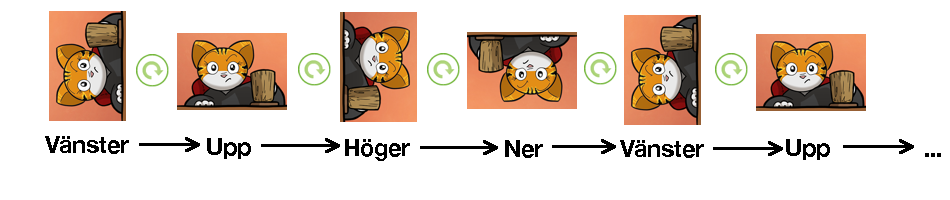
\includegraphics[width=0.8\textwidth]{fotografen.png}
\caption{How an image is rotated}
\label{fig:rotatingcat}
\end{figure}


The photographer thinks rotating photos seems tedious and decides to
turn it into a fun game. The photographer chooses a positive integer $k$ and
decides that the only way to rotate photos is to select exactly $k$ consecutive photos
from the list and rotate all of them simultaneously. Formally, the photographer has $N$ photos, call them $a_1, a_2, \dots
a_N$. The photographer can now choose an index $i$ ($1 \leq i \leq N-k+1$)
and the images $a_i, a_{i+1}, ... , a_{i+k-1}$ are then rotated $90^\circ$ clockwise. We call this an
operation.

The goal of the game is to orient all photos correctly with as few operations as
possible. Write a program that computes the minimum number of operations required.

\section*{Input}
The first line contains two integers $N$ and $k$ ($1 \leq k \leq N \leq 4 \cdot 10 ^5$),
the total number of photos and the number of photos that must be rotated simultaneously.

The second line contains $N$ characters representing the initial rotation of the photographs:
\texttt{U} for up, \texttt{H} for right, \texttt{N} for down, and
\texttt{V} for left.

\section*{Output}
Output the minimum number of operations required. If it is not possible to orient
all photos correctly, output $-1$.

\section*{Scoring}
Your solution will be tested on a set of test groups.
To earn points for a group, you must pass all test cases in that group.

\noindent
\begin{tabular}{| l | l | l |}
  \hline
  \textbf{Group} & \textbf{Points} & \textbf{Constraints} \\ \hline
  $1$   & $10$       & $N \leq 10$ \\ \hline
  $2$   & $40$       & $N \leq 5000$ \\ \hline
  $3$   & $50$       & No additional constraints. \\ \hline
\end{tabular}

\section*{Explanation of Sample 1}
One possible optimal solution is: rotate three times at position 3--4 to get \texttt{UVVU}, then rotate
once at position 2--3 to finally get \texttt{UUUU}, and we are done with four operations.
